De Local Group Policy Editor\index{local group policy editor}\index{gpe}\index{mmc!group policy editor}\index{mmc!gpe}\index{mmc!local group policy editor} (Lokale groepsbeleidsobjecteditor\index{lokale groepsbeleidsobjecteditor}\index{groepsbeleidsobjecteditor}\index{mmc!lokale groepsbeleidsobjecteditor}\index{mmc!groepsbeleidsobjecteditor}) is een MMC snap-in. De Local Group Policy Editor kan gebruikt worden om lokaal settings te zetten voor een bepaalde gebruiker en computer zonder dat dit andere gebruikers of computers hindert op het netwerk.

Er kunnen vele instellingen aangepast worden via de GPEditor, zoals beveilingsopties, systeemgedrag, gebruikersinstellingen, etc. Het wijzigen van deze instellingen is handig voor systemen die niet onderdeel zijn van een domein. In netwerken met een Active Directory domein worden de settings gewoonlijk beheerd door een IT-afdeling via Group Policies (Global Group Policies) of via een MDM-oplossing (Mobile Device Management).

\textbf{Note}: Dit is niet beschikbaar in de Windows Home-edition


Om Computer Management te openen zijn er verschillende manieren:
\begin{itemize}
\item
	\begin{enumerate}
		\item Start MMC
		\item Selecteer in het File menu Add/Remove snap-in
		\item Selecteer Group Policy Objects en klik op Add
		\item Voor de lokale machine selecteer Finish
	\end{enumerate}
\item Gebruik de windows-toets + r en run gpedit.msc\index{gpedit.msc}
\item Klik op het zoek icoon en zoek op Edit Group Policy
\end{itemize}

\begin{minipage}[t]{\linewidth}
\raggedright
\adjustbox{valign=t}{%
	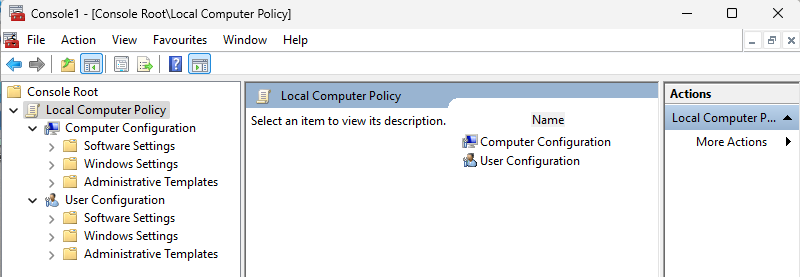
\includegraphics[width=0.99\linewidth]{gpe.png}%
}
\end{minipage}

